\documentclass[a4paper,norsk]{article}
\usepackage{preamble}

\begin{document}
\maketitle
\section*{Assignment i}
In this assignment we are to verify the analytical solutions of the Hagen-Poiseuille Flow for different ducts, presented in White[7]. The ducts to be computed, are an Equilateral triangle, an Ellipse and an Eccentric annulus. I have used the gmsh software to make the different meshes to be calculated. 
\subsection*{Triangle} 
White presents the analythical solution of Hagen-Poiseuille flow over the Equilateral triangle with sides a to be: 

\begin{align*}
	u(y,z) = \frac{\frac{-dp}{dx}}{2*\sqrt{3}a\mu}\Big(z-\frac{1}{2}a\sqrt{3}\Big)
	(3y^2-z^2)
\end{align*}

I have constructed a Fenics program with some defined functions that takes the arguments:
\begin{itemize}
\item{} mesh point size
\item{} a number n that says how many times we want to divide the size of the mesh point
\item{}highest Lagrange order to be calculated. 
\end{itemize}  

Which are used to make the different meshes and controls the number of iterations we do. For example by choosing n to be 3 and the highest Lagrange to be 2, my program will make 2 meshes, and calculate both meshes 2 times. \newline I have used n = 4, highest order of Lagrange to be 3, and mesh point size to be 0.4 in my iteration.

\begin{lstlisting}[style=terminal]
h=9.17E-02 Error=3.33E-04 r=1.27
h=9.17E-02 Error=6.74E-06 r=2.37
h=9.17E-02 Error=2.48E-08 r=-2.13
h=5.90E-02 Error=1.72E-04 r=1.50
h=5.90E-02 Error=2.30E-06 r=2.44
h=5.90E-02 Error=2.17E-08 r=0.31
h=4.15E-02 Error=9.89E-05 r=1.58
h=4.15E-02 Error=9.38E-07 r=2.56
h=4.15E-02 Error=2.26E-08 r=-0.12
\end{lstlisting}

Even though I used the Listing(4) to comupte the error, from my understanding the logarithmic difference seems rather jumpy and not very stable. \newline The error on the other hand seems to be right, due to the descending value of mesh sizes and errors, with the increasing Lagrange degree. So it seems that the proposed analythical solution is correct.

\newpage

\newpage

\subsection*{Ellipse}
For the Ellipse, the suggested analythical solution is presented as:

\begin{align*}
	u(y,z) = \frac{1}{2\mu}\Big(-\frac{dp}{dx} \Big) \frac{a^2b^2}{a^2+b^2} \Big( 1- \frac{y^2}{b^2}-\frac{z^2}{b^2} \Big)
\end{align*}

For the Ellipse, my program is changed slightly by changing the makeel function to make an ellipse, rather than a triangle:
\begin{lstlisting}[style=python]
def makeel(filen, cl):
	file = open(filen, "w")

	file.write("cl = %s;\n" % cl) 
	file.write("Point(2) = {0, 0, 0, cl};\n\
	Point(3) = {-2, 0, 0, cl};\n\
	Point(4) = {2, 0, 0, cl};\n\
	Point(5) = {0, 1, 0, cl};\n\
	Point(6) = {0, -1, 0, cl};\n\
	Ellipse(1) = {6, 2, 4, 4};\n\
	Ellipse(2) = {4, 2, 5, 5};\n\
	Ellipse(3) = {5, 2, 3, 3};\n\
	Ellipse(4) = {3, 2, 6, 6};\n\
	Line Loop(6) = {3, 4, 1, 2};\n\
	Plane Surface(6) = {6};")
	file.close
\end{lstlisting}
Again I have used n = 4, highest order of Lagrange to be 3, and mesh point size to be 0.4 in my iteration. The output yields:

\begin{lstlisting}[style=terminal]
h=8.15E-02 Error=7.48E-05 r=2.08
h=8.15E-02 Error=3.40E-05 r=2.03
h=8.15E-02 Error=3.35E-05 r=2.02
h=4.98E-02 Error=3.28E-05 r=1.67
h=4.98E-02 Error=1.54E-05 r=1.61
h=4.98E-02 Error=1.53E-05 r=1.60
h=3.85E-02 Error=1.95E-05 r=2.03
h=3.85E-02 Error=8.73E-06 r=2.20
h=3.85E-02 Error=8.68E-06 r=2.19
\end{lstlisting}
In this run, I'm more satisfied with the print due to the logarithmic difference is more or less stable. At the same time we observe the error decreases with the mesh size, and the increasing degree of the Lagrange.
\newpage
\lstinputlisting[style=python]{mand1/Triangle/triangle.py}  
\newpage

\section*{Assigment ii}
In this assigment we are to solve to dimentionless equations, one for plane stagnation flow and one for Axisymmetric stagnation flow. 

\subsection*{Stagnation flow}
We obtain the dimensionless equation (146):
\begin{align*}
	F''' + FF'' + 1 -F'^2 = 0
\end{align*}
By defining $ H = F'$ and applying this on the equation we end up with a solveable system.
\begin{align*}
	H-F'+H''+FH'+1-H^2 = 0
\end{align*}
To variational form
\begin{align*}
	\int_{\Omega}^{} (Hv_f-F'v_f+H''v_n+FH'v_n+v_n-H^2v_n)dx 
\end{align*}
The surface integrals goes to zero, hence:
\begin{align*}
	\int_{\Omega}^{}Hv_fdx-\int_{\Omega}^{}\nabla Fv_fdx-
	\int_{\Omega}^{}\nabla h \cdot \nabla v_h dx + \int_{\Omega}^{}F\nabla H v_n dx +
	\int_{\Omega}^{}v_ndx -\int_{\Omega}^{}H^2 v_ndx = 0
\end{align*}


We solve the non-linear equation with Newton and Piccard iterations. The Result har show below for the 


\subsection*{Axisymmetric stagnation flow}
In this situation we obtain the almoust same dimensionless equation, except for the second term which is doubled. Hence we should not get to different plots from this situation, as the graphs show us below. I will not add the code to this sub-exercise due to it's almoust identicall to the stagnation flow.
\begin{align*}
	F''' + 2FF'' + 1 -F'^2 = 0
\end{align*}

\begin{figure}	
	\centering
	\caption*{Equation 146 Newton F}

	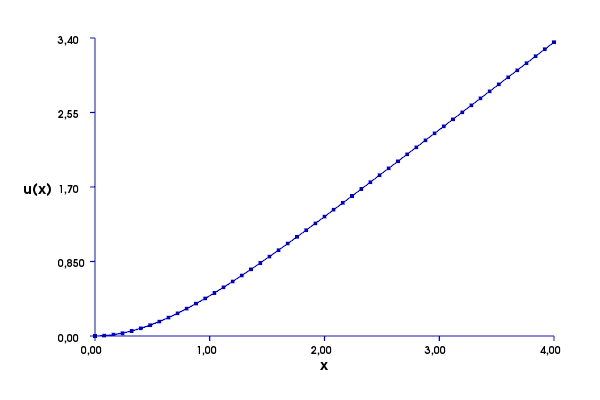
\includegraphics[scale=0.6]{mand2/146newton1.png}
	\caption*{Equation 146 Newtin H}
	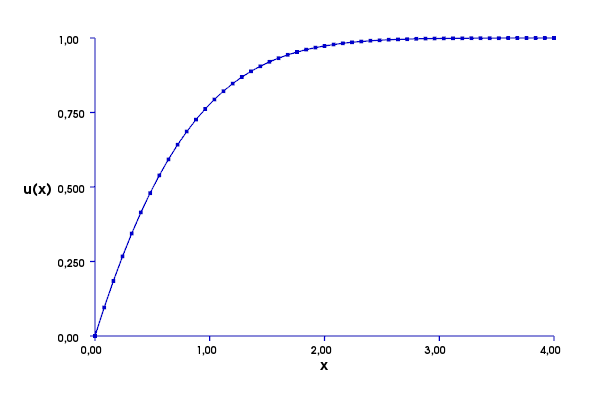
\includegraphics[scale=0.6]{mand2/146newton2.png}
\end{figure}
\begin{figure}	
	\centering
	\caption*{Equation 146 Piccard F}
	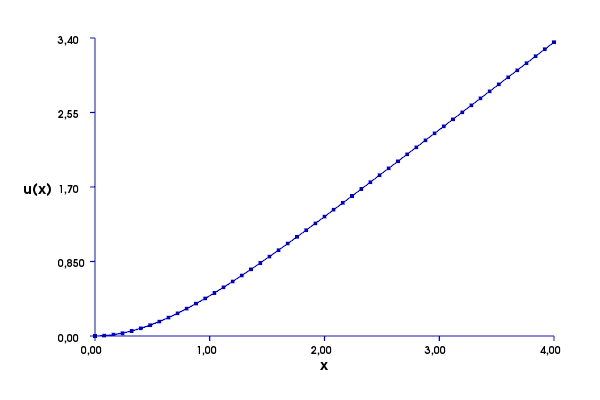
\includegraphics[scale=0.6]{mand2/146picard1.png}
	\caption*{Equation 146 Piccard H}
	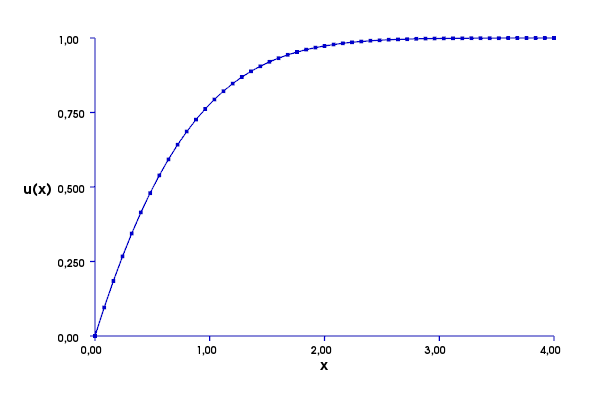
\includegraphics[scale=0.6]{mand2/146picard2.png}
\end{figure}

\begin{figure}	
	\centering
	\caption*{Equation 148 Newton F}
	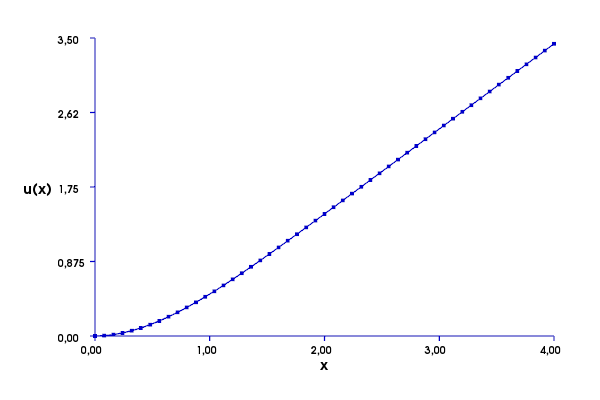
\includegraphics[scale=0.6]{mand2/148newton1.png}
	\caption*{Equation 148 Newton H}
	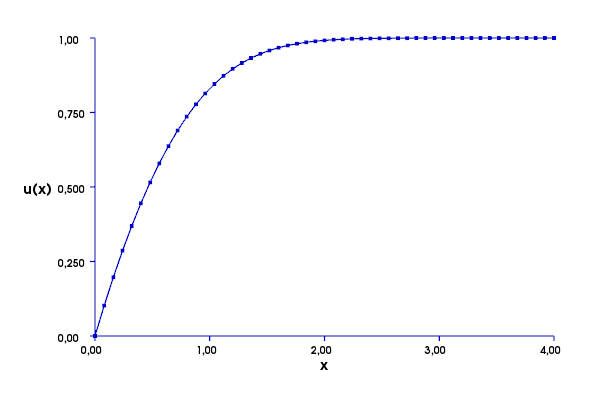
\includegraphics[scale=0.6]{mand2/148newton2.png}
\end{figure}

\begin{figure}	
	\centering
	\caption*{Equation 148 Piccard F}
	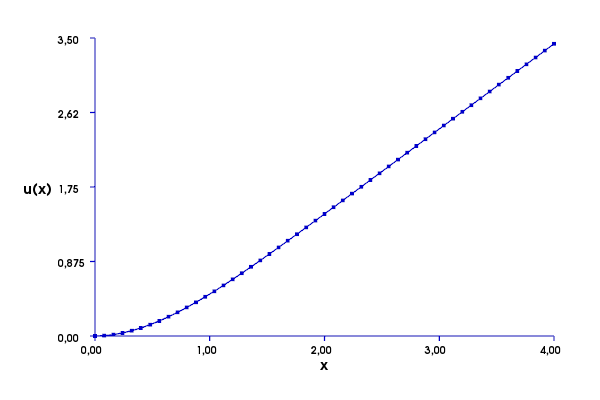
\includegraphics[scale=0.6]{mand2/148picard1.png}
	\caption*{Equation 148 Newton H}
	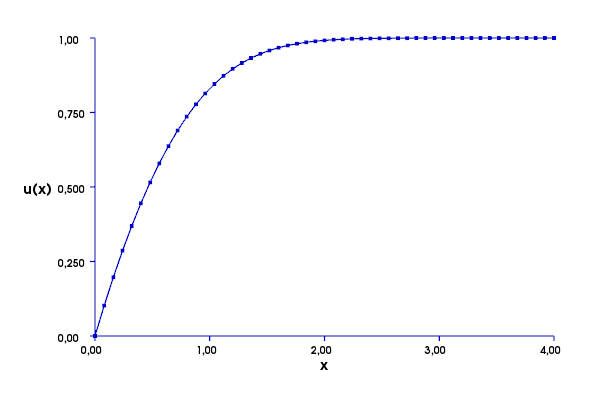
\includegraphics[scale=0.6]{mand2/148picard2.png}
\end{figure}
\newpage
\lstinputlisting[style=python]{mand2/task146.py}
\newpage

\section*{Assignment iii}
In this assignment we are to work with Stokes flow. Assuming low Reynoldnumber the navier-stokes and continuity equations are reduced to:

\begin{align*}
	\mu\nabla^2\textbf{u} = \nabla p \\
	\nabla \cdotp \textbf{u} = 0
\end{align*}
By applying two test functions v and q, we end up with the variational forms for the equation:

\begin{align*}
\int_{\Gamma}^{}\textbf{v} \cdot(\nabla \textbf{u}\cdot \textbf{n})ds -\mu \int_{\Omega}^{} \nabla \textbf{v}:\nabla \textbf{u} dx = \int_{\Gamma}^{}\textbf{v} \cdot p \textbf{n} ds
  - \int_{\Omega}^{}p\nabla \cdot \textbf{v}dx \\
\int_{\Omega}{}q\nabla \cdot \textbf{u} dx = 0
\end{align*}
By summing up the surface integral we get $\int_{\Omega}{} \textbf{v} \cdot (p \textbf{I}- \mu \nabla \textbf{u}) \cdot{n} ds$ which we recognize as the total surface stress. In this case, the surface stress is zero due to pseudo-traction condition.
Running my program I get the following results.

\begin{lstlisting}[style=terminal]
Solving linear variational problem.
[ 0.2  0.3]
\end{lstlisting} 
I have really made an effort to correct my code to get the right coordinates for the vortex. It's clear that this has to be wrong according to my plot, but the plot itself is right. 


\begin{figure}[h!]	
	\centering
	\caption*{Equation Stokes Flow}
	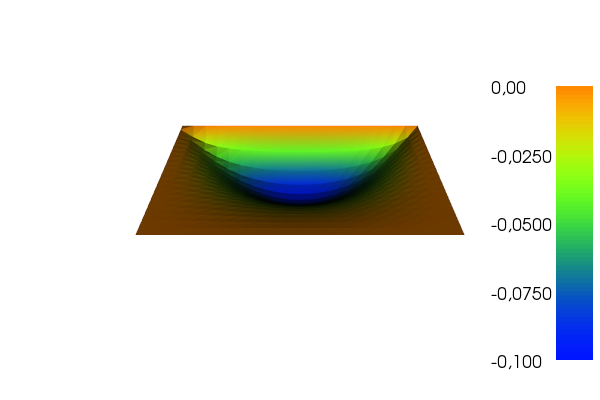
\includegraphics[scale=0.4]{mand3/stokes.png}
\end{figure}
\newpage
\begin{figure}[h!]	
	\centering
	\caption*{Equation Stokes Flow}
	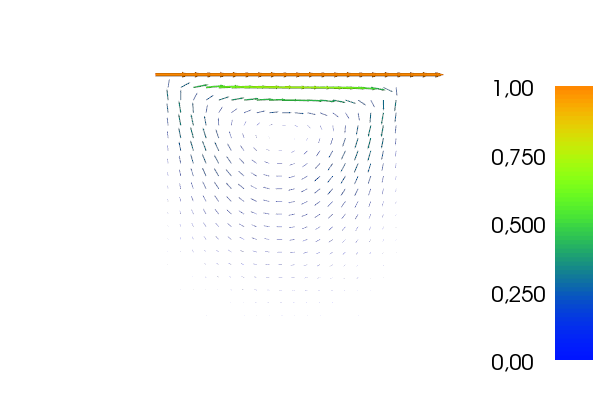
\includegraphics[scale=0.4]{mand3/stokes1.png}
\end{figure}

\lstinputlisting[style=python]{mand3/stokes.py}

\newpage{}


\section*{Assignment iv}
In this assignment we are also looking at Stokes flow. This time we have another mesh as shown in Figure(9). We also apply boundary conditions weakly, the shear stress is added in the variational formulation. The code is more or less the same as the assignment (iii), but with different mesh and variational form. We end up with the following output, code is provided.

\begin{figure}[h!]	
	\centering
	\caption*{Streamfunction}
	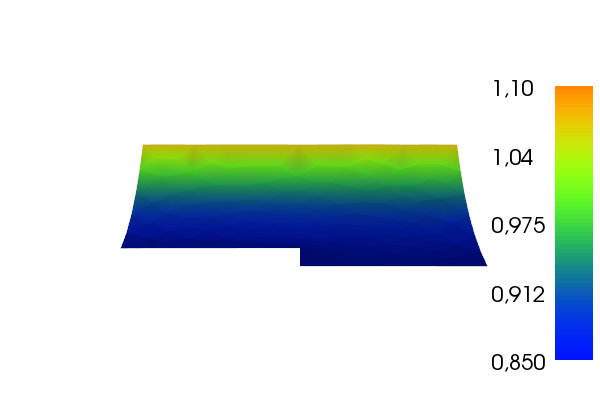
\includegraphics[scale=0.4]{mand4/stokesa.png}
\end{figure}

\begin{lstlisting}[style=terminal]
[[ 0.93508224  0.05647593]]
\end{lstlisting}
Again, clearly my location of the vortex is wrong. It should have a coordinate around 0.52 and 0.1 something. For some reason the code does not provide me the right returned values, so I guess it has something to do with my version.


\subsection*{b)}
Using paraview I get the following plot
\begin{figure}[h!]	
	\centering
	\caption*{Streamfunction}
	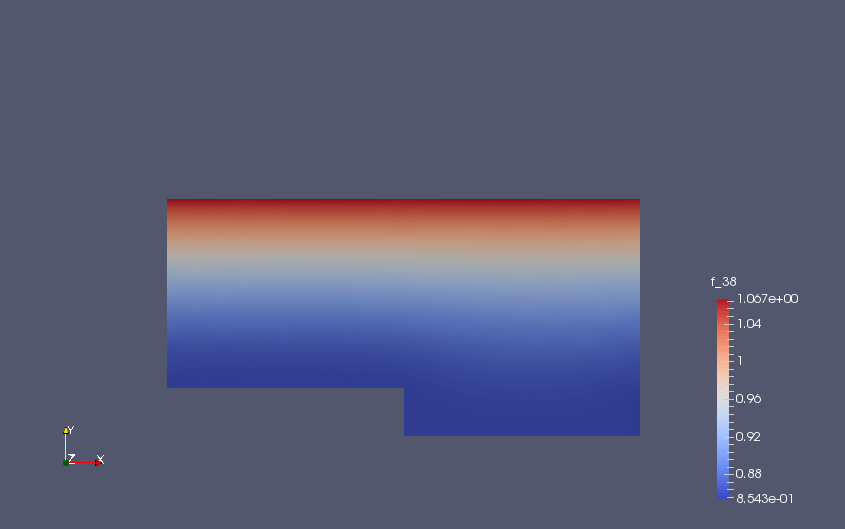
\includegraphics[scale=0.4]{mand4/taskb.png}
\end{figure}
\newpage

\subsection*{c)}
By using the provided code, I'm able to compute the flow through the left and right boundaries.

\begin{lstlisting}[style=terminal]
The flux on the left boundary is -1.165734e-15
The flux on the right boundary is 1.165734e-15
\end{lstlisting}
It seems very well that the mass is being conserved in this system.

\subsection*{d)}
Here we are supposed to reverse the direction of flow in the top boundary to $ \textbf{u} = (-1,0)$. Again since I had some trouble with getting the right coordinates for the vortex center, I'm sure that my code is somewhat right due to I get the following results:

\begin{lstlisting}[style=terminal]
[[ 0.93508224  0.05647593]]
\end{lstlisting}
So even if my point is wrong, it doesn't change. And so due to my results and also by some intuition, the vortex center doesn't change as the top boundary condition change direction. 

\subsection*{e)}
Since we applied weak boundary condition, the shear stress on the boundary is not zero. We compute:
\begin{align*}
	\int_{\Gamma}{}(\gamma \cdot \textbf{n}) \cdot \textbf{n} ds
\end{align*}

\begin{lstlisting}[style=python]
tau = -p_*Identity(2) + mu*(grad(u_) + grad(u_).T)

Bottom = AutoSubDomain(bottom)
mf.set_all(0)
Bottom.mark(mf, 1)

shear = assemble(dot(dot(tau, n), n)*ds, exterior_facet_domains=mf)
print shear
\end{lstlisting}
Which gives us the result:
\begin{lstlisting}[style=terminal]
122.635483966
\end{lstlisting}
By turning the direction of the flow, the result turns negative, so the value of the stress stays the same, but the direction changes. 
\newpage
\lstinputlisting[style=python]{mand4/stokes.py}

\end{document}


